\chapter{Data}
\thispagestyle{empty}

\begin{itemize}
    \item \textcolor{red}{How exactly was data reduced? Use a tikz flowchart}
    \item \textcolor{red}{use mask}
    \item \textcolor{red}{flux/luminosity mask}
    \item \textcolor{red}{AGN mask}
    \item \textcolor{red}{bolometric flux 80\% completeness}
    \item \textcolor{red}{lum vs z image of the reduction steps}
    \item \textcolor{red}{UVJ analysis}
\end{itemize}

\section{The ZFOURGE Survey}
\subsection{Overview} \label{Sec: ZFOURGE Overview}
Our analysis is based on galaxies from the 2017 release\footnote{\href{http://vizier.cds.unistra.fr/viz-bin/VizieR?-source=J/ApJ/830/51&-to=2}{Click here for ZFOURGE Data}} of the ZFOURGE survey \citep{straatman_fourstar_2016}. ZFOURGE consists of approximately 70,000 galaxies at redshifts greater than 0.1 encompassing the three major 11$\times$11 arcminute fields: the Chandra Deep Field South (CDFS), located at coordinates RA: 10h 00m 31s and DEC: $+02^\circ 17' 03"$ \citep{giacconi_chandra_2002}; the Cosmic Evolution Survey (COSMOS), located at RA: 03h 32m 27s and DEC: $-27^\circ 45' 52"$ \citep{scoville_cosmic_2007}, and the CANDELS Ultra Deep Survey (UDS), located at RA: 02h 17m 15s and DEC: $-05^\circ 11' 53"$ \citep{lawrence_ukirt_2007}. These galaxies were observed using the near-infrared FourStar imager \citep{persson_fourstar_2013} mounted on the 6.5-m Magellan Baade Telescope at the Las Campanas Observatory in Chile. ZFOURGE employs deep near-infrared imaging in multiple medium-band filters (\textit{J}$_{1}$, \textit{J}$_2$, \textit{J}$_{3}$, \textit{H}$_{l}$, \textit{H}$_{s}$) and a broad-band \textit{K}$_{s}$ filter. The imaging spans 1.0 to 1.8 $\mu$m and achieves 5$\sigma$ point-source limiting depths of 26 AB mag in the \textit{J} medium-bands and 25 AB mag in the \textit{H} and \textit{K}$_{s}$ bands \citep{spitler_first_2012}. These filters yield well-constrained photometric redshifts, particularly effective for sources within the redshift range of 1 to 4 \citep{spitler_first_2012}. ZFOURGE data is supplemented by public data from HST/WFC3 F160W and F125W imaging from the CANDELS survey, as well as data from Spitzer/Infrared Array Camera (IRAC) and Herschel/Photodetector Array Camera and Spectrometer (PACS). For a detailed description of the data and methodology, refer to \cite{straatman_fourstar_2016}.

\subsection{Sample Selection}
To ensure a comprehensive selection of candidate galaxies and minimise errors, we apply the \texttt{Use=1} criterion as defined in \cite{straatman_fourstar_2016}. This selects a subset of galaxies that meet specific quality requirements, ensuring reliable photometry and redshift measurements. This helps maintain consistency and accuracy in the sample selection process. By employing the \texttt{Use=1} criteria, our sample reduces to 37,647 galaxies. Additionally, we remove any sources with bad or non-existent values to further reduce our sample to 22,967 sources. Finally, we use the ZFOURGE AGN catalogues provided by \cite{cowley_zfourge_2016} to remove 552 AGN dominated sources from our sample, giving us our final sample of 22,444 galaxies. Our reduced ZFOURGE survey spans $0<z<6$ as only 28 galaxies greater than $z=6$ exist in our reduced dataset, so we limit our analysis to a maximum redshift of $z=6$. This data range enables us to observe the evolution of galaxies during some of the most critical cosmic periods, specifically around $1 < z < 3$ \citep{gruppioni_modelling_2011, wylezalek_galaxy_2014} where galaxy luminosity density peaks \citep{assef_mid-ir-_2011}. 

\subfile{Flow Chart}

\begin{figure}[t]
    \centering
    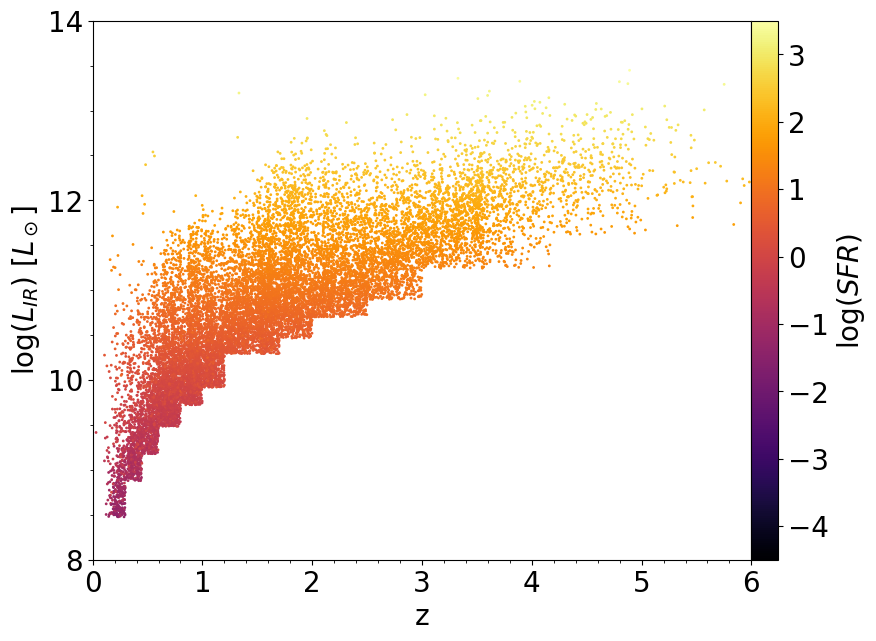
\includegraphics[width=\linewidth]{Figures/ZFOURGE Luminosity Distribution.png}
    \caption{New ZFOURGE Luminosity Distribution following sample selection.}
    \label{Fig: New ZFOURGE Luminosity Distribution}
\end{figure}

\begin{figure}[t]
    \centering
    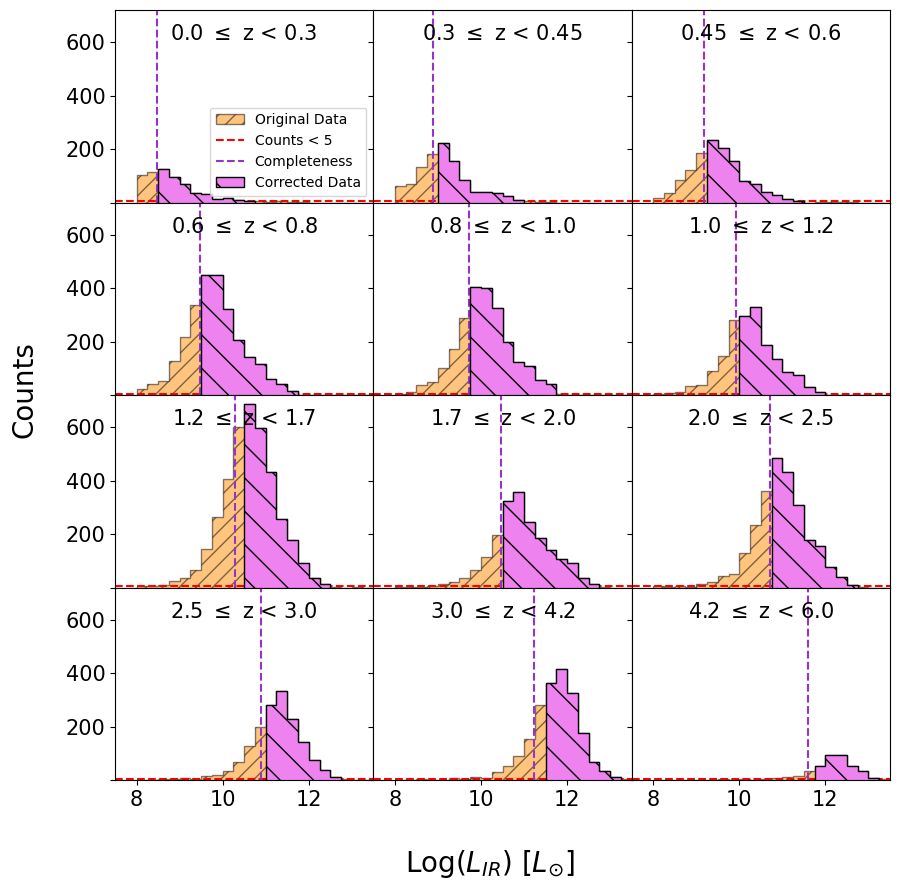
\includegraphics[width=\linewidth]{Figures/ZFOURGE Luminosity Binning.png}
    \caption{ZFOURGE galaxies binned by redshift and luminosity.}
    \label{Fig: ZFOURGE Binned}
\end{figure}

\lipsum[1-3]